%% Draft v0, 2026-11-03. Target: Combustion and Flame (Elsevier, elsarticle).
%% Items marked \todo{} must be resolved before submission. Every reference in refs.bib must be
%% checked against the original paper before submission.
\documentclass[preprint,review,12pt]{elsarticle}

\usepackage[T1]{fontenc}
\usepackage{lmodern}
\usepackage{amsmath,amssymb}
\usepackage{graphicx}
\usepackage{booktabs}
\usepackage{siunitx}
\usepackage{lineno}
\usepackage{xcolor}
\usepackage[hidelinks]{hyperref}
\newcommand{\todo}[1]{\textcolor{red}{[TODO: #1]}}
\newcommand{\pending}[1]{\textcolor{orange}{#1}}
\sisetup{group-separator={\,},group-minimum-digits=4}
\linenumbers
\journal{Combustion and Flame}

\begin{document}
\begin{frontmatter}

\title{State or increment? The output of neural-network chemistry surrogates decides which part of
a reacting flow they get right}

\author[a]{Javier \todo{surname}}
\author[a]{\todo{co-authors}}
\address[a]{\todo{affiliation}}

\begin{abstract}
Neural-network surrogates of finite-rate chemistry are trained either to predict the thermochemical
state at the end of the chemistry step, usually in a transformed space that stretches small mass
fractions, or to predict the physical increments $\Delta Y_k$ and $\Delta T$. The choice is often
treated as an implementation detail. We compare the two outputs with everything else fixed: the same
residual network with FiLM conditioning, the same a priori training data, the same online learning
scheme (ISANN, in which the running simulation fine-tunes the surrogate on its own direct
integrations), the same laminar methane/air burner with an 18-species mechanism in OpenFOAM, and the
same machine. In the flame ($T>1600$~K) both outputs are equally good: the mean temperature error
against direct integration is 1.3--3.7~K for the increment output and 1.8--2.5~K for the state
output from 25 to 50~ms, and both keep total CO and OH within 5\% of direct integration. Outside the flame they differ by orders of magnitude.
In the lean burnt gas that fills most of the hot volume (1300--1600~K), the increment-output network
leaves 16 times the CO, 2.5 times the OH and about 100 times the H of direct integration, and the gas
runs 2--5~K cold; the state output keeps them within a factor 1.5 and the temperature within 0.4~K. The cause is the loss
scaling: there, the CO increment per step is $2\times10^{-3}$ of its global standard deviation in
physical units but 0.2 in Box--Cox units, so the physical-increment loss weights these states
$\sim10^4$ times less than the flame. Conversely, the increment output is better where the state
output is weak: an offline Cantera benchmark shows 2--5 times less temperature drift at equilibrium and
in lean hot gas. In the online scheme the increment output also kept 10 times more hot cells on direct integration
(1.4--2.5\% against 0.04--0.33\%), which made it 1.5 times slower per step. We conclude that the output parametrisation and its loss
scaling must be chosen for the region of composition space that matters for the application, and
that a priori one-step errors averaged over the data do not reveal the difference.
\end{abstract}

\begin{keyword}
Chemistry acceleration \sep Neural network surrogate \sep Output parametrisation \sep Loss scaling
\sep Box--Cox transformation \sep Online learning
\end{keyword}
\end{frontmatter}

%% ===============================================================================================
\section{Introduction}
\label{sec:intro}

Artificial neural networks (ANN) have been used to replace the stiff integration of chemical source
terms since the 1990s~\cite{christo1996ann,blasco1998ann}, with training data from similar
simulations~\cite{sen2010les}, canonical flames~\cite{ihme2009ann}, or abstract problems that sample
composition space~\cite{franke2017rcce,ding2021hybrid,readshaw2021hybrid}, and more recently as
neural ordinary differential equations~\cite{owoyele2022chemnode}. Whatever the data, the network has
to return the state at the end of a chemistry step of length $\Delta t$, and there are two common ways
to do it:
\begin{itemize}
\item \emph{State output}: the network predicts the end state $Y(t+\Delta t)$, usually as a residual
  on the start state in a transformed space. A Box--Cox or logarithmic transformation~\cite{boxcox1964}
  stretches the small mass fractions of radicals and intermediates, so that their relative accuracy
  counts in the loss.
\item \emph{Increment output}: the network predicts the physical increments $\Delta Y_k$ (and
  $\Delta T$), each standardised by its own scale over the training data. This is the form of a
  reaction-rate or source-term regression and makes the zero increment at equilibrium trivial to
  represent.
\end{itemize}
Both forms appear in the literature \todo{cite examples of each: e.g.\ \cite{franke2017rcce,ding2021hybrid}
predict increments of standardised (log/BCT) variables; source-term regressions; check each paper's
exact output and scaling before citing}, but we are not aware of a controlled comparison in a
reacting-flow simulation, where the surrogate is called in a chain and its errors accumulate.
\todo{literature check of comparisons of output parametrisation for chemistry ANNs.}

This paper isolates that choice. We take a surrogate that we use in an online learning scheme,
ISANN~\cite{isann2026}, in which a simulation starts with direct integration (DI), trains the network on
its own DI results, and switches to it once it passes an acceptance gate. We then change only the
output layer and the loss of the network, from the next Box--Cox state to the physical increments,
and repeat the same simulation from the same state on the same machine. The comparison covers the
CFD solution against DI (temperature, CO, OH, H by region), the course of the online training, the
share of cells sent back to DI, the cost, and an offline benchmark on Cantera states that does not
depend on the CFD.

The contributions are: (i) a controlled comparison of the two outputs in a laminar methane/air burner
with an 18-species mechanism; (ii) the identification of the loss scaling, not the network, as the
cause of the difference, with a direct measurement of the increment sizes in both units; (iii) the
observation that the two outputs fail in complementary regions, which suggests how to combine them.

%% ===============================================================================================
\section{Surrogate model}
\label{sec:model}

\subsection{Network}
The network maps the composition at the start of a chemistry step to the end of the step at constant
pressure and enthalpy. The species mass fractions are Box--Cox transformed ($\lambda=0.1$),
\begin{equation}
  \tilde y_k = \frac{Y_k^{\lambda}-1}{\lambda},
\end{equation}
and standardised to $y_k=(\tilde y_k-\mu_k)/s_k$; the context $c=(T,\,p,\,h,\,\log_{10}\Delta t)$ is
standardised in the same way. The network is a residual MLP whose blocks are modulated by the context
through feature-wise linear modulation (FiLM)~\cite{perez2018film}: an input layer, three residual
blocks of 192 units with layer normalisation and SiLU activations, and a linear output layer $W_o z+b_o$
initialised to zero (about $2.4\times10^5$ parameters). Steps longer than the trained range
($\Delta t=$ \num{1e-5}--\num{4e-5}~s) are sub-stepped, and cells below $T_\mathrm{freeze}=600$~K
are not advanced. After every step the composition is projected onto non-negative mass fractions that
sum to one, and the temperature follows from the conserved enthalpy by Newton iteration.

\subsection{The two outputs}
\paragraph{State output (Y)} The output is a residual in the standardised Box--Cox space,
\begin{equation}
  \hat y(t+\Delta t) = y(t) + W_o z + b_o ,
\end{equation}
decoded to $\hat Y_k$. The one-step loss is on the predicted increment in that space, scaled per species
by $\sigma_{\Delta y,k}$, the standard deviation of the Box--Cox increments over the training data:
\begin{equation}
  L_Y = \Big\langle \sum_k \Big(\frac{\hat y_k(t+\Delta t)-y_k(t+\Delta t)}{\sigma_{\Delta y,k}}\Big)^2\Big\rangle .
  \label{eq:lossY}
\end{equation}

\paragraph{Increment output (dY)} The output layer has $N_s+1$ outputs, the physical increments scaled by
their standard deviations over the training data, $\sigma_{\Delta Y,k}$ and $\sigma_{\Delta T}$:
\begin{equation}
  \hat Y_k(t+\Delta t) = Y_k(t) + \sigma_{\Delta Y,k}\,(W_o z+b_o)_k,\qquad
  \hat T_\mathrm{net} = T(t) + \sigma_{\Delta T}\,(W_o z+b_o)_{N_s+1},
\end{equation}
and the one-step loss is
\begin{equation}
  L_{\Delta Y} = \Big\langle \sum_k \Big(\frac{\hat Y_k(t+\Delta t)-Y_k(t+\Delta t)}{\sigma_{\Delta Y,k}}\Big)^2\Big\rangle .
  \label{eq:lossdY}
\end{equation}
The temperature term of the loss averages the error of the enthalpy temperature and of
$\hat T_\mathrm{net}$. OpenFOAM and Ansys Fluent compute the temperature from the transported enthalpy
and take only the species from the chemistry step, so $\hat T_\mathrm{net}$ is trained and reported but
not used by the CFD. Both networks also have the same multi-step rollout loss on 8-step Cantera
segments and the same push-forward noise.

The two losses differ only in the units in which an error is measured. In Box--Cox units, $d\tilde y_k
= Y_k^{\lambda-1}dY_k$, so a given absolute error $dY_k$ counts $Y_k^{\lambda-1}$ times more where the
species is scarce: for CO at $Y=10^{-4}$ the factor is $(10^{-2}/10^{-4})^{0.9}\approx63$ times larger
than at $Y=10^{-2}$. In physical units, every state of a species has the same weight per
unit of $dY_k$, so the states with the largest increments, i.e.\ the flame, dominate.

\subsection{Training}
The state-output parent (\emph{ood7}) was trained on states obtained without any CFD solution: 0D
ignition and equilibrium relaxation, partially stirred reactors, steady and unsteady flamelets over
a range of strain rates, vitiated, heat-loss and burnt-gas relaxation variants, at the inlet
conditions of the burner \todo{numbers of pairs per regime; cite the exploration paper}. The
increment-output parent (\emph{ood7dy}) takes the trunk (input layer and residual blocks) of ood7, a new
zero-initialised output layer of $N_s+1$ outputs, and is trained for 80 epochs (one-cycle learning rate
up to \num{1e-3}, noise amplitude 0.005, rollout loss weight 0.2) on the same a priori data; its
validation temperature error is 0.12~K per step. \todo{Control for the extra 80 epochs: fine-tune ood7
with the state output for the same 80 epochs.}

\subsection{Online learning (ISANN)}
Both parents are then used in the same ISANN run~\cite{isann2026}, with identical criteria. The run
starts with DI (GA18 mechanism, seulex) in every cell and stores the (state, $\Delta t$, DI result)
pairs after a two-level deduplication. The first network is trained when the store saturates or at
step 400 at the latest. A trainer process fine-tunes the current network (20 epochs, peak learning rate
\num{2e-4}) on the online pairs plus three times as many a priori pairs (replay), and an acceptance gate
on 15\% held-out online pairs (one-step $|\Delta T|$ must improve; 120 100-step 0D rollouts against
Cantera must not get worse) decides whether all ranks switch to it. After the switch, cells flagged as
out of distribution (OOD) and cells of temperature--mixture-fraction bins where a sparse shadow DI
check finds the network wrong ($|T-T_\mathrm{DI}|>\max(1~\mathrm{K},0.3|\Delta T_\mathrm{DI}|)$ or the same
for OH with a floor of \num{5e-5}) are integrated with DI and produce new pairs. A new round starts
after 1500 new pairs, a DI share above 5\%, or an untrusted bin, up to 12 rounds. Each network keeps its
output form through the rounds.

%% ===============================================================================================
\section{Test case and comparison}
\label{sec:case}

The burner is a laminar non-premixed methane/air burner of domestic cooking geometry, computed
2D axisymmetric (60k cells) with rhoReactingBuoyantFoam (OpenFOAM v2412, Euler implicit,
$\Delta t=\num{2e-5}$~s, 2 MPI ranks) and the GA18 skeletal mechanism (18 species) \todo{GA18 reference}.
Pure CH$_4$ enters at 300~K through a central tube, air through an annular co-flow, and a pot with
convective walls sits above the burner. The simulation starts from a lit state, lean ($\phi=0.5$)
burnt gas at 1480~K in the gap under the pot and air elsewhere, and is run for 50~ms; the reference is
a DI run from the same state \todo{geometry figure, as in \cite{isann2026}}.

Both ISANN runs were made one after the other in the same container (4 cores, 2 for the CFD and 2 for
the trainer), so their costs are comparable. A state-output run with the same settings had been made
earlier on another machine~\cite{isann2026}; we show it for reproducibility.

\paragraph{Metrics} Snapshots are compared with DI every 2.5~ms: the mean $|T-T_\mathrm{DI}|$ in the
flame zone ($T>1600$~K in either solution) and over all hot cells ($T>600$~K); the mean relative error
of OH and CO over the hot cells where the DI value exceeds $10^{-3}$ of its maximum; and, by
temperature band, the mean $T-T_\mathrm{DI}$ and the ratio of the integrated mass of CO, OH and H to that
of DI. \paragraph{Offline benchmark} 218 physics-only Cantera states in six families (equilibrium,
cooled products, lean hot gas, vitiated mixtures, partially burnt mixtures, counterflow flamelets) are
advanced as constant-$(p,h)$ reactors for 2500 steps of \num{2e-5}~s through the same C code as the CFD,
with the surrogate on every step, and compared with Cantera.

%% ===============================================================================================
\section{Results}
\label{sec:results}

\subsection{Accuracy against direct integration}
Figure~\ref{fig:time} and Table~\ref{tab:summary} compare the two runs. In the flame zone the increment
output is as good as the state output: 1.3--3.7~K from 25 to 50~ms against 1.8--2.5~K, with
practically no bias in either. Over all hot cells it is three times worse (3.1--5.1~K against 0.8--1.7~K),
and its mean relative errors of OH (138--179\% against 19--68\%) and CO (57--84\% against 18--28\%) are
about three times those of the state output. The state-output run reproduces the flame and OH errors of
the earlier run on another machine~\cite{isann2026} but not its CO error (18--28\% against 4--7\%): the two
runs accepted different networks at different times (first network at 9.1 against 11.2~ms), which
gives an idea of the run-to-run spread of the online scheme.

\begin{figure}[t]
\centering
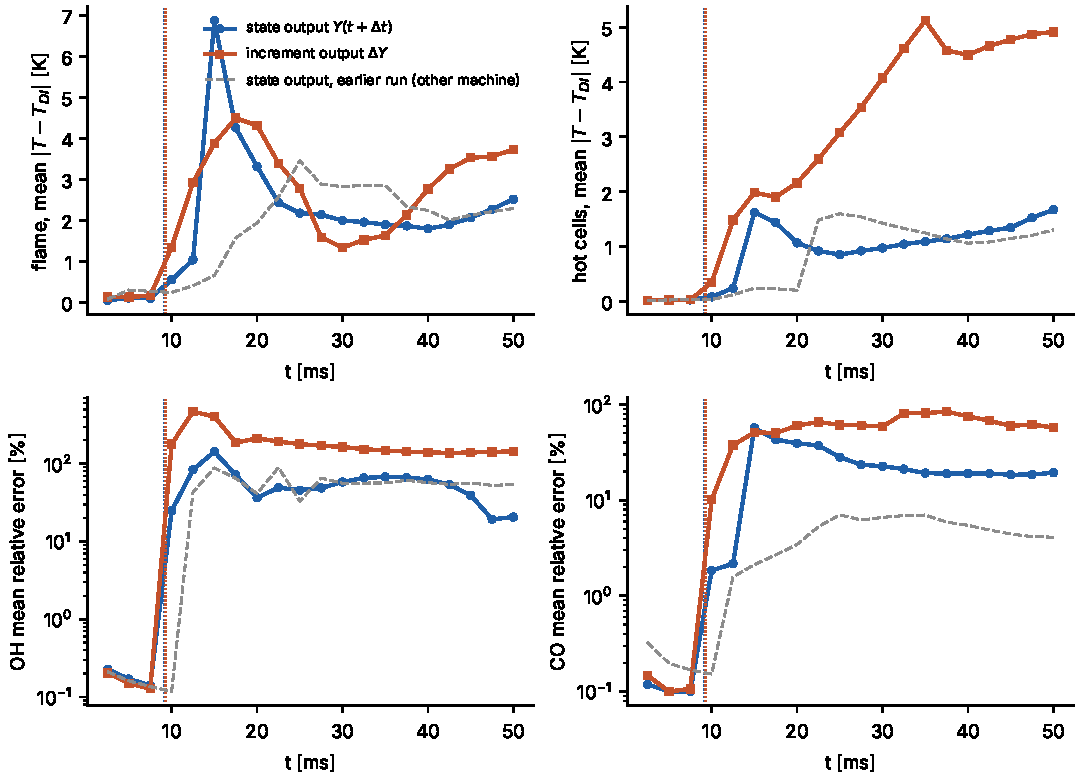
\includegraphics[width=\textwidth]{figs/fig_accuracy_time.pdf}
\caption{Error against DI during the two ISANN runs. Dotted vertical lines: first network in use.
Grey dashed: the state-output run made earlier on another machine~\cite{isann2026}.}
\label{fig:time}
\end{figure}

\begin{table}[t]
\centering
\caption{The two outputs in the same ISANN run (25--50~ms unless stated).}
\label{tab:summary}
\small
\begin{tabular}{lcc}
\toprule
 & State $Y(t+\Delta t)$ & Increment $\Delta Y$ \\
\midrule
First network in use [ms] & 9.1 & 9.3 \\
Networks accepted / rounds & 5 / 9 & 6 / 12 \\
Flame mean $|T-T_\mathrm{DI}|$ [K] & 1.8--2.5 & 1.3--3.7 \\
Hot-cell mean $|T-T_\mathrm{DI}|$ [K] & 0.8--1.7 & 3.1--5.1 \\
OH mean relative error [\%] & 19--68 & 138--179 \\
CO mean relative error [\%] & 18--28 & 57--84 \\
Hot cells on DI, network phase [\%] & 0.04--0.33 & 1.4--2.5 \\
Wall time per step, network phase [s] & 2.8--3.2 & 4.2--4.7 \\
Wall time per step, DI phase [s] & 5.4 & 5.2 \\
\bottomrule
\end{tabular}
\end{table}

Figure~\ref{fig:bands} locates the difference. Above 1600~K the increment-output run has the CO, OH and
H of DI within 2\% (CO 0.98, OH 0.98, H 0.99 times DI at 50~ms). Below 1600~K it does not: at 50~ms the
integrated CO is 30, 7.9 and 16 times that of DI in the bands 600--1000, 1000--1300 and 1300--1600~K,
OH 15, 4.2 and 2.5 times, and H 99, 350 and 97 times; the band 1300--1600~K holds \num{36000} of the
\num{44000} hot cells, the lean burnt gas under the pot. That gas is 2--5~K colder than DI, consistent
with CO that is not oxidised. Figure~\ref{fig:comaps} shows that the CO excess covers the whole burnt-gas
region except the flame around the fuel jet. The state output keeps the band 1300--1600~K within
0.4~K of DI, with CO 1.5, OH 0.98 and H 1.2 times DI. Both outputs are poor in the coolest gas
(600--1300~K, 6400 cells), close to $T_\mathrm{freeze}$ and in the mixing layer with the air: there the
state output is 3--12~K cold, with CO 3.5--4 times and OH 0.04 times DI, and the increment output has CO
8--30 times, OH 4--15 times and H 100--350 times DI.

\begin{figure}[t]
\centering
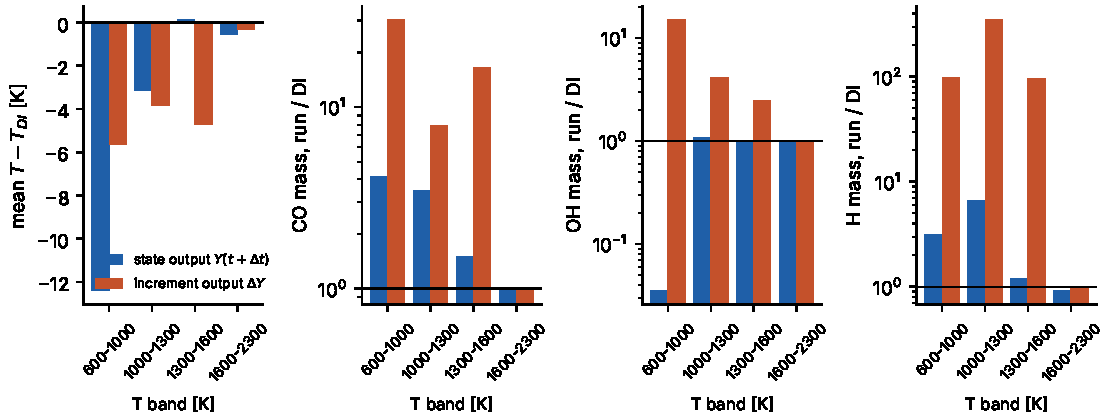
\includegraphics[width=\textwidth]{figs/fig_bands.pdf}
\caption{Error by temperature band at 50~ms: mean temperature bias, and integrated mass of CO, OH and H
relative to DI (1 = exact; logarithmic axis).}
\label{fig:bands}
\end{figure}

\begin{figure}[t]
\centering
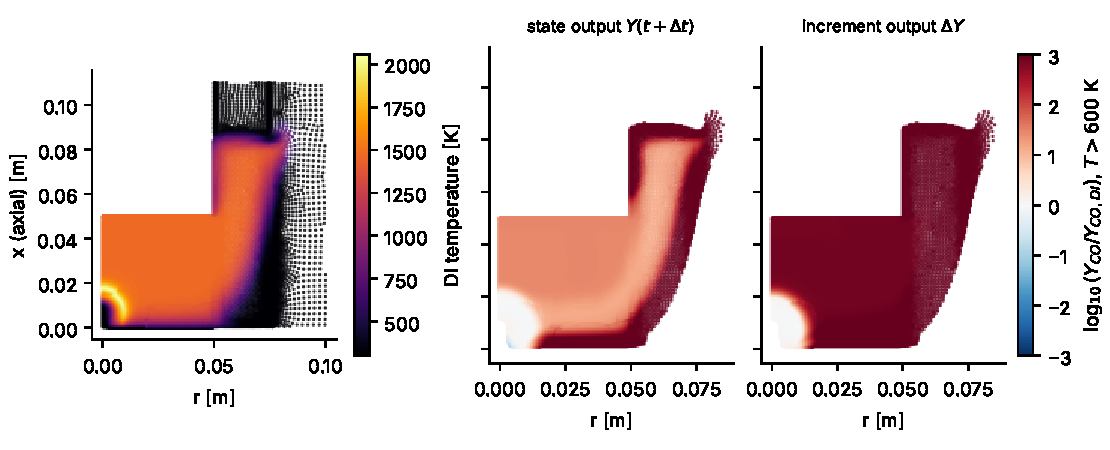
\includegraphics[width=\textwidth]{figs/fig_co_maps.pdf}
\caption{Left: DI temperature at 50~ms in the region under and beside the pot. Right:
$\log_{10}$ of the CO mass fraction of each run relative to DI, in cells above 600~K.}
\label{fig:comaps}
\end{figure}

\subsection{Why: the size of the increments in each loss}
Table~\ref{tab:scales} measures the increment per step of the DI pairs of the run, in the units of each
loss (Eqs.~\ref{eq:lossY} and~\ref{eq:lossdY}). In the flame, the CO increment is 0.38 of its scale in
physical units and 1.1 in Box--Cox units: both losses see it. In the lean burnt gas (1300--1600~K) it
is $2.4\times10^{-3}$ of its scale in physical units but 0.22 in Box--Cox units. Relative to the flame,
the squared loss therefore weights these states $(0.38/0.0024)^2\approx2.5\times10^4$ times less with the
increment output and $(1.1/0.22)^2\approx25$ times less with the state output. With CO at
$\sim10^{-4}$ and OH at $\sim10^{-4}$, an error of a few $10^{-6}$ per step is invisible to
$L_{\Delta Y}$, but over the $\sim10^3$ steps a parcel spends in this gas it is what decides whether the
CO burns out. The same holds for OH and, much more strongly, for H (Table~\ref{tab:scales}).

\begin{table}[t]
\centering
\caption{Median per-step increment of the DI pairs of the run, in units of the scale of each loss:
$|\Delta Y_k|/\sigma_{\Delta Y,k}$ (increment output) and $|\Delta y_k|/\sigma_{\Delta y,k}$ (state output,
Box--Cox). \num{126997} pairs.}
\label{tab:scales}
\small
\begin{tabular}{llrrr}
\toprule
$T$ band [K] & Species & median $Y_k$ & $|\Delta Y_k|/\sigma_{\Delta Y,k}$ & $|\Delta y_k|/\sigma_{\Delta y,k}$ \\
\midrule
600--1300 & CO & \num{7.9e-05} & \num{5.6e-04} & \num{3.4e-02} \\
 & OH & \num{3.9e-06} & \num{1.0e-03} & \num{1.2e-01} \\
 & H & \num{2.7e-10} & \num{2.6e-04} & \num{5.7e-01} \\
 & CO$_2$ & \num{7.7e-02} & \num{2.2e-04} & \num{1.8e-04} \\
\addlinespace
1300--1600 & CO & \num{1.1e-04} & \num{2.4e-03} & \num{2.2e-01} \\
 & OH & \num{7.2e-05} & \num{3.6e-03} & \num{3.0e-02} \\
 & H & \num{8.4e-08} & \num{3.5e-03} & \num{2.1e-01} \\
 & CO$_2$ & \num{7.8e-02} & \num{2.0e-03} & \num{1.1e-03} \\
\addlinespace
1600--2300 & CO & \num{1.0e-02} & \num{3.8e-01} & \num{1.1e+00} \\
 & OH & \num{9.1e-04} & \num{1.3e-01} & \num{1.2e-01} \\
 & H & \num{1.0e-05} & \num{9.0e-02} & \num{1.3e-01} \\
 & CO$_2$ & \num{1.2e-01} & \num{2.5e-01} & \num{1.0e-01} \\
\bottomrule
\end{tabular}
\end{table}

The shadow check, which compares single steps with absolute floors, does not see this either: the
increment-output run had 1.4--2.5\% of the hot cells in untrusted bins on DI, about ten times the state
output (Figure~\ref{fig:share}), but the error builds up over many steps that each pass the check.

\subsection{Offline benchmark}
Figure~\ref{fig:bench} shows the networks on the Cantera states, with no CFD involved. The increment
output is better for temperature where nothing should happen: at equilibrium the mean temperature drift
after 50~ms is 36~K against 82~K for ood7, and in lean hot gas 9.6~K against 52~K, because a zero
increment is a zero output for this network but a residual that must cancel exactly in Box--Cox space
for the other. It is worse for the radicals in every family: the median error of H after 1~ms is a
factor $10^{1.07}$ against $10^{0.17}$ overall, and $10^{3.25}$ against $10^{0.33}$ in lean hot gas. The online rounds
reduce the radical errors of both outputs but not the gap (H: $10^{0.63}$ against $10^{0.16}$ for the final
networks), and they remove the temperature error in lean hot gas for both (0.15 and 0.32~K), the states
the burner is full of. They also move the equilibrium drift apart: the final increment-output network
drifts by 28~K, the final state-output network by 135~K, a region the burner does not visit. In the CFD only the species matter, because the temperature comes from the
enthalpy, so the temperature advantage of the increment output is not used and its radical error is.

\begin{figure}[t]
\centering
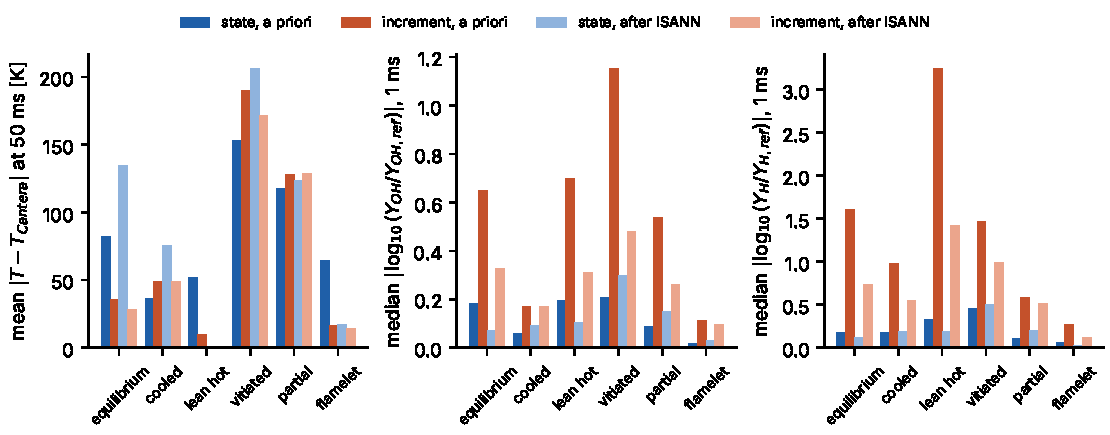
\includegraphics[width=\textwidth]{figs/fig_benchmark.pdf}
\caption{Offline benchmark on 218 Cantera states, surrogate alone: temperature error after 50~ms and
radical errors after 1~ms, by family, for the two parents and the final networks of the two ISANN runs.}
\label{fig:bench}
\end{figure}

\subsection{Online training and cost}
The increment-output run switched to its first
network at 9.3~ms (round 1 accepted) and accepted 6 networks in 12 rounds; rounds 5, 7, 8 and 11
returned the current network unchanged, the same plateau seen with the state output~\cite{isann2026}.
The wall time per step with the network was 4.2--4.7~s against 5.2~s in the DI phase
(Figure~\ref{fig:share}); most of the remaining cost is the flow solver and the DI of the cells kept on
DI. The state-output run accepted 5 networks in 9 rounds (rounds 6--9 rejected, the run ended before
round 10) and ran at 2.8--3.2~s per step with the network against 5.4~s in the DI phase. The difference in
cost between the two runs is the share of cells on DI: 0.04--0.33\% of the hot cells for the state output
and 1.4--2.5\% for the increment output, whose shadow checks kept more bins untrusted.

\begin{figure}[t]
\centering
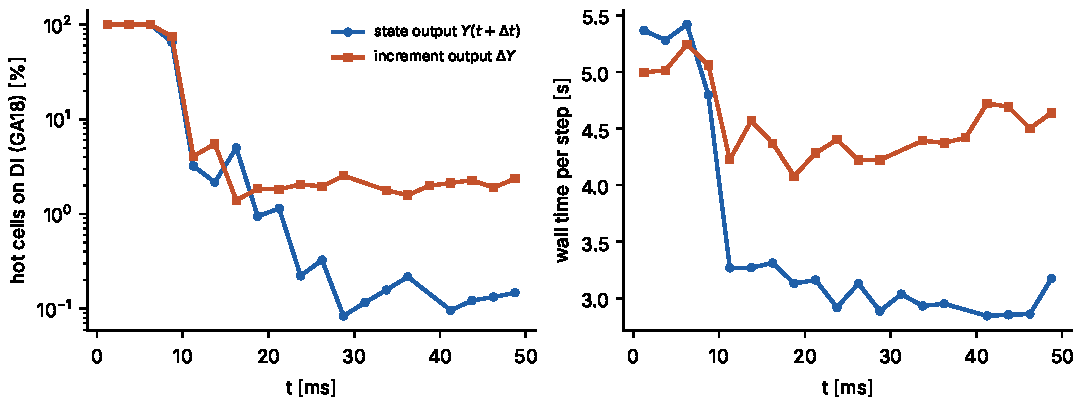
\includegraphics[width=\textwidth]{figs/fig_share_cost.pdf}
\caption{Share of hot cells integrated with DI and wall time per step (2.5~ms windows).}
\label{fig:share}
\end{figure}

%% ===============================================================================================
\section{Discussion}
\label{sec:discussion}

\paragraph{What the output decides} The two networks have the same architecture, data and online
scheme, and their temperature errors in the flame are the same. What the output changes is the
\emph{weight of each region of composition space in the loss}. A state output in a stretched space gives
the scarce species of the near-equilibrium burnt gas a weight comparable to the flame; a physical
increment output gives the flame almost all the weight. In a burner where most hot gas is lean burnt gas,
that decides the CO and radical levels of most of the domain.

\paragraph{One-step metrics hide it} The a priori validation error of the increment output (0.12~K per
step) is as good as that of the state output, and on the run's own DI pairs its one-step temperature
error was lower (0.74 against 1.13~K) while its relative OH, CO and H errors were 3--6 times worse. Data
averages are dominated by the states with large increments; region-resolved and multi-step metrics are
needed to see the difference.

\paragraph{Combining the two} The failures are complementary: the increment output keeps equilibrium
and lean hot gas at the right temperature, the state output keeps the minor species. Options are a loss
on physical increments scaled per species and per state, e.g.\ by $\max(|\Delta Y_k|,\epsilon Y_k)$
instead of a global $\sigma_{\Delta Y,k}$; a two-term loss on increments and on the next Box--Cox state; or
an increment output in Box--Cox space, which is what the state output already is. \todo{test one of them
in the same protocol.}

\paragraph{Limitations} One burner, one mechanism, one training seed per output, and the increment-output
parent had 80 more epochs of training than the state-output parent. The relative errors depend on
the floor used for scarce species. Temperature comes from the enthalpy in both solvers, which removes one
possible advantage of the increment output.

%% ===============================================================================================
\section{Conclusions}
\label{sec:conclusions}

With everything else fixed, replacing the next-state output of a chemistry surrogate by a physical
increment output left the flame equally accurate but multiplied CO by 8--30 and OH by 2.5--15 in the
lean burnt gas around it, needed ten times more cells on direct integration in an online scheme (and
so 1.5 times more time per step), and made the hot-cell temperature error three times larger. The cause is the loss scaling, which in physical
units makes the small increments of near-equilibrium gas invisible. The increment output was better
only for the temperature at equilibrium, which the CFD does not take from the network. Output form and
loss scaling should therefore be chosen, and evaluated, region by region.

\section*{Data and code availability}
Code: \url{https://github.com/jaba09/chemmanifold-studio} (option \texttt{model.output: dY}, OpenFOAM
ISANN in \texttt{openfoam/isann}, figures in \texttt{papers/y-vs-dy}). \todo{archive with DOI.}

\section*{Acknowledgements}
\todo{}

\bibliographystyle{elsarticle-num}
\bibliography{refs}

\end{document}
